%=====================================================================
%  IEEE journal manuscript. Compile with pdfLaTeX + BibTeX
%  Order:  pdfLaTeX -> BibTeX -> pdfLaTeX -> pdfLaTeX
%  Multimodal polysomnography: joint staging + respiratory-event detection.
%  Supervision draft: full benchmark, math formulation, expanded review.
%=====================================================================
\documentclass[journal]{IEEEtran}
\IEEEoverridecommandlockouts
\usepackage{cite}
\usepackage{amsmath,amssymb,amsfonts}
\usepackage{algorithmic}
\usepackage{graphicx}
\usepackage{textcomp}
\usepackage{xcolor}
\usepackage{booktabs}
\usepackage{array}
\usepackage{multirow}
\usepackage{url}
\usepackage{stfloats}   % lets two-column (starred) floats sit at the bottom of a page
% allow more (and wider) floats per page so the many two-column tables place near
% their references instead of piling up after the bibliography.
\setcounter{topnumber}{3}
\setcounter{totalnumber}{5}
\setcounter{dbltopnumber}{3}
\renewcommand{\topfraction}{0.95}
\renewcommand{\bottomfraction}{0.7}
\renewcommand{\dbltopfraction}{0.95}
\renewcommand{\textfraction}{0.05}
\renewcommand{\floatpagefraction}{0.7}
\renewcommand{\dblfloatpagefraction}{0.7}
\def\BibTeX{{\rm B\kern-.05em{\sc i\kern-.025em b}\kern-.08em T\kern-.1667em\lower.7ex\hbox{E}\kern-.125emX}}

% Headline numbers (results/mm_final_cv.json).
\newcommand{\mmAcc}{0.721}
\newcommand{\mmMf}{0.645}
\newcommand{\mmK}{0.606}
\newcommand{\mmAuc}{0.700}
\newcommand{\mmAp}{0.333}
\newcommand{\eegAuc}{0.655}
\newcommand{\noflowAuc}{0.707}

\begin{document}

\title{Multimodal Polysomnography for Joint Sleep Staging and Respiratory-Event Detection in Subacute Ischemic Stroke}

\author{Md Wahiduzzaman Sua, Esm-e Moula Chowdhury Abha, and Md Imtiaj Alam Sajin%
\thanks{The authors are with the Department of Computer Science and Engineering,
American International University-Bangladesh, Dhaka, Bangladesh
(e-mail: 26-94088-2@student.aiub.edu; 26-94089-2@student.aiub.edu;
26-94090-2@student.aiub.edu).}}

\markboth{Manuscript, July 2026}%
{Sua \MakeLowercase{\textit{et al.}}: Multimodal Polysomnography in Ischemic Stroke}

\maketitle

%=====================================================================
\begin{abstract}
A clinical polysomnogram records far more than the brain. Alongside the
electroencephalogram it captures eye movements, muscle tone, the electrocardiogram,
nasal and oral airflow, thoracic and abdominal breathing effort, and blood oxygen
saturation. In patients recovering from ischemic stroke, a group in which breathing is
disturbed during sleep at high rates, these cardiorespiratory signals carry the disease
itself. We build one model that reads the full polysomnogram and produces two clinical
outputs at once: the sleep stage of every 30-second epoch and a per-epoch label for
respiratory events. The model encodes the neural and the cardiorespiratory signals in two
parallel streams, lets the two streams exchange information through cross-modal attention,
follows the night with a bidirectional recurrent decoder, and drives a staging head and a
respiratory head, with a direct connection that carries the cardiorespiratory signal to the
respiratory head so oxygen desaturation reaches the decision at full strength. We benchmark
the model against fifteen architectures on iSLEEPS, the first public polysomnography corpus
of subacute ischemic stroke (99 patients), all under patient-independent ten-fold
cross-validation. The single model stages sleep at $\mmAcc$ accuracy with Cohen's $\kappa$
of $\mmK$, which places it among the strongest models on this cohort, and it detects
respiratory events at $\mmAuc$ area under the ROC curve, a capability none of the staging
models possess. The respiratory read-out is grounded in physiology: when we remove the
airflow channel from which the events were scored, detection holds at $\noflowAuc$, because
the model reads oxygen desaturation, breathing effort, cardiac variability, and the cortical
arousals that follow an obstructed breath. Each modality contributes where its physiology
lives. Code and features are released.
\end{abstract}

\begin{IEEEkeywords}
Polysomnography, multimodal learning, sleep staging, sleep apnea, ischemic stroke,
cross-modal attention, multi-task learning, cardiorespiratory signals.
\end{IEEEkeywords}

%=====================================================================
\section{Introduction}
\IEEEPARstart{S}{leep} is scored in 30-second epochs into five stages, Wake (W), N1, N2,
N3, and rapid-eye-movement (REM), following the American Academy of Sleep Medicine (AASM)
rules~\cite{aasm2023manual}. The overwhelming majority of automated methods read a single
electroencephalogram (EEG) channel and ask one question: how accurately can the five stages
be classified? Two decades of work on that question have moved from convolutional and
recurrent encoders~\cite{supratak2017deepsleepnet,phan2019seqsleepnet,supratak2020tinysleepnet}
through attention and sequence models~\cite{eldele2021attnsleep,phan2021xsleepnet,
perslev2019utime} to large self-supervised EEG foundation
models~\cite{labram2024,cbramod2025,eegpt2024,biot2023}. On healthy sleepers these methods
reach roughly $85\%$ accuracy, and recent reviews argue the field is near a ceiling set by
inter-scorer disagreement~\cite{phan2022survey}.

A clinical polysomnogram (PSG), however, is a recording of the whole sleeping body. It
carries the EEG, eye movements, muscle tone, the electrocardiogram (ECG), nasal and oral
airflow, thoracic and abdominal breathing effort, and peripheral oxygen saturation
(SpO$_2$). These cardiorespiratory channels are where sleep-disordered breathing writes
itself: a paused breath, a chest that keeps straining against a closed airway, a fall in
blood oxygen, and the arousal that rescues the breath. A model that reads only the EEG
cannot see any of this, and so cannot report on the disorder that most damages a patient's
sleep. We use the full polysomnogram, and we ask a question that the staging race does not:
what does a model gain, and on which clinical task, when it reads the whole recording rather
than the brain alone.

We study this on iSLEEPS~\cite{maiti2026isleeps}, released in 2026 as the first public PSG
corpus dedicated to subacute ischemic stroke. The cohort is well matched to the question.
Sleep-disordered breathing is common in the weeks after a stroke and is tied to worse
recovery~\cite{bassetti2006sleep,denis2024sleep}, and in this corpus the median patient
carries a scored respiratory event in $13\%$ of epochs, with $77$ of $96$ patients above
$5\%$ (Fig.~\ref{fig:prev}). The cardiorespiratory signal is therefore abundant and
clinically meaningful in exactly the population where breathing matters most. The published
staging baselines on this corpus reach $74.7\%$ accuracy for an LSTM, about ten points below
the healthy state of the art, and a concurrent study reports that deep networks attend to
non-physiological regions on this cohort~\cite{bose2026gap}, so the setting also stresses
every staging architecture we can bring to it.

We present a two-stream, multi-task model that treats staging and respiratory-event
detection as one joint problem, and we place it inside a broad benchmark of fifteen
architectures on the same folds. Our contributions are:

\begin{itemize}
\item \textbf{One model for two clinical read-outs from the full polysomnogram.} It stages
sleep at $\mmAcc$ accuracy ($\kappa$ $\mmK$) and, from the same forward pass, detects
respiratory events at $\mmAuc$ AUC, with a direct cardiorespiratory path to the respiratory
head so oxygen-desaturation cues reach the decision undiminished (Section~\ref{sec:method}).
\item \textbf{A broad benchmark on the stroke cohort.} We compare against convolutional,
recurrent, transfer-learned, foundation-style, graph, gradient-boosting, and stacking models,
all under patient-independent ten-fold evaluation (Table~\ref{tab:bench}). Staging saturates
near $0.72$ to $0.75$ across every strong architecture, and the proposed model sits inside
that band while adding a respiratory capability the others lack.
\item \textbf{A respiratory read-out grounded in physiology, not in the labeling signal.}
Removing the airflow channel from which the events were scored leaves detection at
$\noflowAuc$ AUC, because the decision rests on oxygen desaturation, breathing effort,
cardiac variability, and cortical arousals (Section~\ref{sec:noflow}).
\end{itemize}

%=====================================================================
\section{Related Work}
\label{sec:related}

\subsection{Single-channel deep sleep staging}
Automated staging matured on one EEG channel. DeepSleepNet paired convolutional feature
extraction with a bidirectional LSTM~\cite{supratak2017deepsleepnet}; SeqSleepNet framed the
night as sequence-to-sequence labeling~\cite{phan2019seqsleepnet}; AttnSleep introduced
attention over multi-resolution convolutions~\cite{eldele2021attnsleep}; TinySleepNet and
U-Time reduced the parameter budget while holding
accuracy~\cite{supratak2020tinysleepnet,perslev2019utime}; and XSleepNet fused raw and
spectral views~\cite{phan2021xsleepnet}. These models set the accuracy on healthy corpora but
depend on the cortical micro-events that stroke disturbs, which is why they transfer poorly to
patients~\cite{bose2026gap}.

\subsection{Multi-channel and foundation models}
Later work reads several PSG channels. U-Sleep stages from arbitrary EEG and EOG derivations
across many cohorts~\cite{perslev2021usleep}, and self-supervised EEG foundation models such
as LaBraM, CBraMod, EEGPT, and BIOT learn transferable representations from large unlabeled
corpora~\cite{labram2024,cbramod2025,eegpt2024,biot2023}. SleepFM extends this idea to several
PSG modalities~\cite{sleepfm2026}. The eye and muscle channels help most with REM and Wake,
which a single EEG channel resolves poorly. Reported gains from adding respiratory channels to
\emph{staging} are small and cohort-dependent; our benchmark quantifies this directly on a
high-burden clinical cohort and separates the staging effect from the respiratory one.

\subsection{Detection of sleep-disordered breathing}
A parallel line of work detects apnea and hypopnea from breathing signals. Airflow and effort
shape, oximetry, and ECG-derived heart-rate variability are all informative, and oxygen
desaturation is a defining marker of an event~\cite{jing2025cpap}. These detectors usually run
at fine time resolution on the raw breathing waveforms and are trained on that task alone. We
instead detect respiratory events on the staging epoch grid, jointly with staging, from a
shared representation, so that one model produces both clinical outputs and the two tasks
support each other during training.

\subsection{Sleep and breathing after stroke}
Sleep is both disturbed by stroke and predictive of recovery, and sleep-disordered breathing
is common in the subacute phase and linked to poorer functional
outcome~\cite{bassetti2006sleep,denis2024sleep}. Focal injury also changes the micro-events
that scoring relies on, the spindles, slow waves, and muscle
atonia~\cite{gottselig2002stroke,fernandez2019spindles,simpson2023laterality}. A model that
reports on breathing as well as stage is therefore of direct clinical value in this
population.

%=====================================================================
\section{Dataset and Preprocessing}
\label{sec:data}
iSLEEPS~\cite{maiti2026isleeps} contains overnight PSG from 100 subacute ischemic-stroke
patients (mean age $50.5$; 77 male, 23 female), scored by experts into the five AASM stages.
We exclude one recording after an audit: the data records of SN28 are byte-identical to those
of SN15, a duplication consistent with the anonymization and re-numbering the dataset authors
describe, and keeping it would place a training subject into the test fold in nine of ten fold
assignments. We therefore use $N=99$ ($96$ with complete cardiorespiratory channels), a total
of $89{,}532$ epochs. The stage distribution (Table~\ref{tab:dist}) is strongly imbalanced,
with N2 dominant and N1 and N3 scarce, which is the clinical norm.

\begin{table}[t]
\caption{Stage distribution and respiratory-event prevalence in the corpus we model ($N=99$).}
\label{tab:dist}
\centering
\begin{tabular}{lccccc}
\toprule
Stage & W & N1 & N2 & N3 & R \\
\midrule
Share (\%) & 26.6 & 10.2 & 42.3 & 8.9 & 12.1 \\
\bottomrule
\end{tabular}
\\[2pt]
\footnotesize Respiratory events: $16.0\%$ of epochs positive; median $13\%$ per patient
(range $0$ to $60.5\%$); $77$ of $96$ patients above $5\%$.
\end{table}

\begin{figure}[t]
\centering

\includegraphics[width=0.86\columnwidth]{figures/fig_mm_apnea_prev.pdf}
\caption{Sleep-disordered-breathing burden across the cohort. Each bar counts patients by the
fraction of epochs that carry a scored respiratory event. The median patient sits at $13\%$
and many exceed $30\%$, so the cardiorespiratory signal is abundant.}
\label{fig:prev}
\end{figure}

\paragraph{Channels we read, and channels we do not}
A raw recording holds 22 traces. We read the 14 that carry sleep-stage or breathing
information. The \emph{neural stream} takes the four EEG derivations (C4:M1, C3:M2, O2:M1,
O1:M2), the two EOG channels (E1:M2, E2:M2), and the submental EMG. The
\emph{cardiorespiratory stream} takes the ECG, nasal and oral airflow, thoracic effort,
abdominal effort, the summed effort trace, SpO$_2$, and pulse. We leave out eight traces for
stated reasons: periodic limb movement records a different disorder; snore is scored from the
same airway sound as the respiratory events and would make the second task circular;
plethysmography is already summarized by the SpO$_2$ and pulse channels we keep; body position
is coarse and slow; and the ambient-light and battery traces are device housekeeping, not
physiology. All neural channels are resampled to $100$\,Hz and the cardiorespiratory channels
to $25$\,Hz, and both are read in physical units, which matters because SpO$_2$ near $90\%$,
pulse near $78$\,bpm, and microvolt EEG live on very different scales. Per-epoch respiratory
labels are the corpus's scored events mapped onto the $30$\,s grid, and an epoch is positive
when it overlaps an event.

%=====================================================================
\section{Proposed Method}
\label{sec:method}
\subsection{Problem formulation}
A night is a sequence of $T$ epochs. For epoch $t$ we form a neural feature vector
$\mathbf{f}^{\mathrm{eeg}}_t\in\mathbb{R}^{188}$ and a cardiorespiratory feature vector
$\mathbf{f}^{\mathrm{car}}_t\in\mathbb{R}^{14}$, and we learn a subject-independent map
\begin{equation}
f_\theta:\big(\mathbf{f}^{\mathrm{eeg}}_{1:T},\mathbf{f}^{\mathrm{car}}_{1:T}\big)\ \longmapsto\
\big(\hat y^{\mathrm{stg}}_{1:T},\ \hat y^{\mathrm{apn}}_{1:T}\big),
\end{equation}
where $\hat y^{\mathrm{stg}}_t\in\Delta^4$ is a distribution over the five stages and
$\hat y^{\mathrm{apn}}_t\in[0,1]$ is the probability that epoch $t$ contains a respiratory
event (Fig.~\ref{fig:arch}).

\begin{figure*}[t]
\centering

\includegraphics[width=\textwidth]{figures/fig_architecture.pdf}
\caption{The two-stream, multi-task model. (A) The neural features and the cardiorespiratory
features are encoded in parallel, combined by a cross-modal fusion block, and read across the
night by a bidirectional LSTM. A staging head reads the recurrent state; a respiratory head
reads the recurrent state together with a direct copy of the cardiorespiratory embedding, so
oxygen-desaturation and effort cues reach the respiratory decision without passing through the
staging-oriented fusion. (B) Detail of the feature encoder and of the fusion block, which
tokenizes the two modalities, runs four-head attention, and combines the result with a
residual connection.}
\label{fig:arch}
\end{figure*}

\subsection{Physiological feature representations}
\paragraph{Neural features ($188$)}
Per channel we take absolute and relative band powers from the Welch spectrum $P(f)$ in delta
($0.5$--$4$), theta ($4$--$8$), alpha ($8$--$12$), sigma ($12$--$16$), and beta
($16$--$30$)\,Hz; the relative power in band $b$ is
\begin{equation}
\mathrm{RP}_b=\frac{\int_{f\in b}P(f)\,df}{\int_{0.5}^{30}P(f)\,df}.
\end{equation}
We add spectral entropy $H=-\sum_i p_i\log p_i$ with $p_i$ the normalized spectrum, the
$95\%$ spectral-edge frequency, the three Hjorth descriptors~\cite{hjorth1970eeg}, and
time-domain statistics. Sleep spindles are detected on the sigma-band analytic envelope
$e(t)=\lvert\mathcal{H}\{x_\sigma\}(t)\rvert$ from the Hilbert transform $\mathcal{H}$, with
density counted above a per-epoch threshold; slow-wave amplitude, ocular-movement energy on
the EOG, and tonic EMG level complete the set.

\paragraph{Cardiorespiratory features ($14$)}
From the seven cardiorespiratory channels we compute SpO$_2$ mean, minimum, variability, and
desaturation depth (median minus minimum); pulse mean and variability; ECG amplitude and
line-length; airflow amplitude and line-length; thoracic, abdominal, and summed effort
amplitudes; and thoraco-abdominal asynchrony, the loss of coordination between chest and
abdomen that marks an obstructed breath,
\begin{equation}
\mathrm{asyn}_t=\big\lvert\,\mathrm{corr}(x^{\mathrm{tho}}_t,\ x^{\mathrm{abd}}_t)\,\big\rvert .
\end{equation}
Both feature sets are standardized per patient, which removes person-to-person offsets so the
model generalizes across people.

\subsection{Two-stream encoders}
Each stream is a two-layer perceptron with LayerNorm,
\begin{align}
e_t&=\mathrm{GELU}\!\big(\mathrm{LN}(W_2\,\mathrm{GELU}(\mathrm{LN}(W_1\mathbf{f}^{\mathrm{eeg}}_t))) \big)\in\mathbb{R}^{128},\\
c_t&=\mathrm{GELU}\!\big(\mathrm{LN}(U_2\,\mathrm{GELU}(\mathrm{LN}(U_1\mathbf{f}^{\mathrm{car}}_t))) \big)\in\mathbb{R}^{64}.
\end{align}
LayerNorm rather than BatchNorm is used because the recurrent windows are short and mix
patients within a batch, and the cardiorespiratory stream is deliberately narrower because
$14$ slow descriptors carry far less structure than $188$ neural features.

\subsection{Cross-modal fusion}
The two embeddings become two tokens with learned modality-type embeddings
$M\in\mathbb{R}^{2\times D}$, $D=128$,
\begin{equation}
T=\big[\,W_e\,e_t\ ;\ W_c\,c_t\,\big]+M\ \in\ \mathbb{R}^{2\times D}.
\end{equation}
Four-head scaled dot-product attention lets each modality read the other,
\begin{equation}
\mathrm{head}_i=\mathrm{softmax}\!\Big(\tfrac{(TW^Q_i)(TW^K_i)^{\!\top}}{\sqrt{d_k}}\Big)\,TW^V_i,
\quad A=\big[\mathrm{head}_1;\dots;\mathrm{head}_4\big]W^O,
\end{equation}
followed by a residual connection, normalization, and a projection of the two refined tokens,
\begin{equation}
\tilde T=\mathrm{LN}(T+A),\qquad z_t=\mathrm{GELU}\!\big(W_f\,\mathrm{vec}(\tilde T)\big)\in\mathbb{R}^{D}.
\end{equation}
We also evaluate a plain concatenation in place of attention; the two perform alike
(Section~\ref{sec:ablate}), so the reported gain is attributable to the modality, not to the
fusion mechanism.

\subsection{Temporal decoder and two heads}
Sleep is sequential and respiratory events cluster, so the fused vectors of an $L=20$ epoch
window ($10$ minutes) are read by a two-layer bidirectional LSTM. Each direction runs the
standard recurrence
\begin{align}
i_t&=\sigma(W_i[z_t,h_{t-1}]), & f_t&=\sigma(W_f[z_t,h_{t-1}]),\nonumber\\
o_t&=\sigma(W_o[z_t,h_{t-1}]), & g_t&=\tanh(W_g[z_t,h_{t-1}]),\\
s_t&=f_t\odot s_{t-1}+i_t\odot g_t, & h_t&=o_t\odot\tanh(s_t),\nonumber
\end{align}
and the forward and backward states are concatenated into $h_t\in\mathbb{R}^{256}$. The
staging head is a linear map $\hat y^{\mathrm{stg}}_t=\mathrm{softmax}(W_s h_t)$. The
respiratory head reads $h_t$ together with a direct copy of the per-epoch cardiorespiratory
embedding $c_t$,
\begin{equation}
\hat y^{\mathrm{apn}}_t=\sigma\!\big(W_2\,\mathrm{GELU}(W_1[h_t;c_t])\big).
\end{equation}
This direct connection matters: without it the respiratory decision must survive a fusion
trained mostly for staging, and the fall in oxygen that defines an event is weakened along the
way. The full model holds $0.86$ million parameters.

\subsection{Training and decoding}
The two tasks are trained together with equal weight,
\begin{equation}
\mathcal{L}=\underbrace{-\sum_t\sum_{k}w_k\,y^{\mathrm{stg}}_{t,k}\log\hat y^{\mathrm{stg}}_{t,k}}_{\text{staging}}
\ +\ \lambda\underbrace{-\sum_t\big[\pi\,a_t\log\hat y^{\mathrm{apn}}_t+(1{-}a_t)\log(1{-}\hat y^{\mathrm{apn}}_t)\big]}_{\text{respiratory}},
\end{equation}
with $\lambda=1$. The staging weights use the square root of inverse class frequency,
$w_k\propto\sqrt{N/(K n_k)}$ for $K=5$ classes with $n_k$ examples, which corrects the scarce
N1 and N3 stages without giving up overall accuracy, and the respiratory term is
positive-weighted by $\pi=n_-/n_+$ to match the $16\%$ event rate. At inference the staging
posteriors are smoothed by a hidden-Markov Viterbi pass whose transition matrix $A^{\mathrm H}$
and prior are counted from the training labels~\cite{chen2024hmm},
\begin{equation}
\delta_t(j)=\max_i\big[\delta_{t-1}(i)+\log A^{\mathrm H}_{ij}\big]+\log\hat y^{\mathrm{stg}}_t(j),
\end{equation}
recovered by back-tracking, which restores the natural persistence of sleep. The respiratory
head is left unsmoothed. Optimization uses AdamW with cosine annealing and early stopping on a
held-out set of patients.

%=====================================================================
\section{Experiments}
\label{sec:results}
\subsection{Protocol and metrics}
All results use ten-fold, patient-independent cross-validation, so no patient appears in both
training and test, and within each training split a disjoint set of patients is held out for
early stopping. Staging is scored by accuracy, macro-F1 $\tfrac{1}{K}\sum_k\mathrm{F1}_k$, and
Cohen's $\kappa$. The respiratory task is scored by the area under the ROC curve (AUC) and
average precision (AP), which suits the $16\%$ event rate.

\subsection{Compared Methods}
We benchmark the model against a wide set of approaches on the same folds. The \emph{deep}
group holds convolutional and recurrent networks trained from scratch (DeepSleepNet,
AttnSleep, a four-channel CNN with BiLSTM), a network transferred from Sleep-EDF, sequence
CNN-BiLSTM models on four and seven channels, and a raw-signal convolutional network on all
$14$ channels. The \emph{feature} group holds a single gradient-boosting classifier, a
feature-sequence BiLSTM, a learnable refiner, a hemispheric graph-attention model with a
state-space decoder, a stacking ensemble, and a four-member gradient-boosting ensemble. The
published single-channel baselines for the corpus are included for
reference~\cite{maiti2026isleeps}. All numbers are ten-fold patient-independent, at the
hidden-Markov operating point where a model provides one.

\begin{table*}[t]
\caption{Sleep-staging benchmark on iSLEEPS, ten-fold patient-independent. All rows are the
five-class staging task at the hidden-Markov operating point where available. Ch.\ is the
number of input channels; ``feat'' marks engineered features. Best per column in
\textbf{bold}. The proposed model is the only one that also detects respiratory events
(Table~\ref{tab:ablate}).}
\label{tab:bench}
\centering
\setlength{\tabcolsep}{6pt}
\begin{tabular}{llccccc}
\toprule
Model & Group & Input & Params\,$\downarrow$ & Acc\,$\uparrow$ & Macro-F1\,$\uparrow$ & $\kappa$\,$\uparrow$ \\
\midrule
\multicolumn{7}{l}{\emph{Published single-channel baselines}~\cite{maiti2026isleeps}}\\
LSTM                       & recurrent   & 1\,EEG    & --      & 0.747 & 0.677 & 0.640 \\
Transformer                & attention   & 1\,EEG    & --      & 0.674 & 0.594 & 0.540 \\
CNN-ResNet18               & convolution & 1\,EEG    & $\sim$11\,M & 0.617 & 0.544 & 0.480 \\
\midrule
\multicolumn{7}{l}{\emph{Deep models (this study)}}\\
DeepSleepNet~\cite{supratak2017deepsleepnet} & conv+LSTM & 1\,EEG & $\sim$21\,M & 0.615 & 0.567 & 0.483 \\
AttnSleep~\cite{eldele2021attnsleep}         & attention & 1\,EEG & $\sim$0.5\,M & 0.686 & 0.629 & 0.577 \\
CNN\,+\,BiLSTM             & conv+LSTM   & 4\,EEG    & $\sim$0.6\,M & 0.613 & 0.565 & 0.485 \\
Sleep-EDF transfer         & transfer    & 4\,EEG    & $\sim$0.6\,M & 0.623 & 0.582 & 0.488 \\
Sequence CNN-BiLSTM        & conv+LSTM   & 4\,EEG    & $\sim$0.8\,M & 0.645 & 0.609 & 0.526 \\
Sequence CNN-BiLSTM        & conv+LSTM   & 7\,ch     & $\sim$0.8\,M & 0.654 & 0.610 & 0.544 \\
Raw multimodal CNN         & conv+LSTM   & 14\,ch    & 0.95\,M & 0.655 & 0.612 & 0.531 \\
\midrule
\multicolumn{7}{l}{\emph{Feature and ensemble models (this study)}}\\
Gradient boosting (single) & feature     & 7\,ch feat & --     & 0.655 & 0.499 & 0.485 \\
Feature-sequence BiLSTM    & feature     & 7\,ch feat & 1.2\,M & 0.676 & 0.639 & 0.566 \\
Learnable refiner          & feature     & 7\,ch feat & $\sim$0.5\,M & 0.704 & 0.661 & 0.600 \\
Graph attention + SSM      & feature     & 7\,ch feat & 0.49\,M & 0.730 & \textbf{0.703} & 0.633 \\
Stacking ensemble          & feature     & 7\,ch feat & --     & 0.735 & 0.692 & 0.639 \\
Gradient-boosting ensemble & feature     & 7\,ch feat & --     & \textbf{0.746} & 0.675 & \textbf{0.641} \\
\midrule
\multicolumn{7}{l}{\emph{Proposed multimodal multi-task model}}\\
MM-Net (neural only)       & feature     & 7\,ch feat & 0.77\,M & 0.721 & 0.635 & 0.603 \\
\textbf{MM-Net (neural + cardio)} & feature & 14\,ch feat & 0.86\,M & 0.721 & 0.645 & 0.606 \\
\bottomrule
\end{tabular}
\end{table*}

\subsection{Staging Benchmark and Comparison}
Table~\ref{tab:bench} shows a clear pattern. Every raw-signal deep network, whether trained
from scratch or transferred, stays near $0.62$ to $0.66$ accuracy, and the strong feature and
ensemble models cluster between $0.70$ and $0.75$. Staging on this stroke cohort saturates in
that band regardless of architecture, which matches the concurrent finding that depth alone
does not help here~\cite{bose2026gap}. The proposed model stages at $\mmAcc$ accuracy, inside
the top group and above every from-scratch deep network, while using under a million
parameters. What sets it apart is not a staging record but a second output: it is the only
model in the table that also detects respiratory events.

\begin{figure}[t]
\centering
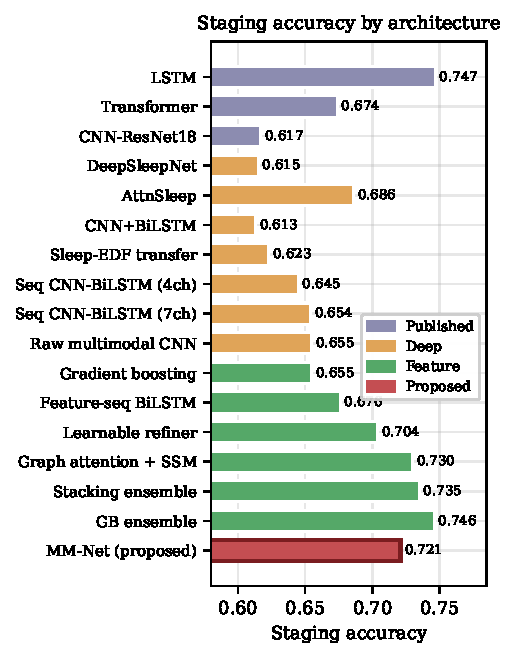
\includegraphics[width=0.94\columnwidth]{figures/fig_benchmark.pdf}
\caption{Staging accuracy across the fifteen benchmarked architectures (ten-fold,
patient-independent), grouped by family. The proposed model sits inside the top band of the
feature and ensemble models while remaining compact.}
\label{fig:benchmark}
\end{figure}

\subsection{Per-class Staging Performance}
Table~\ref{tab:perclass} breaks staging down by stage. The pattern is the one this cohort
imposes on every method: N2, Wake, and REM are recovered well, N3 is moderate, and N1 is the
hard stage for all models, because N1 is transient and rare. The raw convolutional network
reaches the highest N1 F1, which fits its sensitivity to short events, while the
gradient-boosting ensemble leads on the stable stages. The proposed model tracks the strong
feature models across every stage. Per-class scores were not recorded for some baselines and
are marked with a dash.

\begin{table*}[t]
\caption{Per-class staging F1 (Wake, N1, N2, N3, REM) across the compared architectures,
ten-fold patient-independent, at the hidden-Markov operating point. A dash marks a model for
which per-class scores were not recorded in our runs. Best per column in \textbf{bold}.}
\label{tab:perclass}
\centering
\setlength{\tabcolsep}{8pt}
\begin{tabular}{llccccc}
\toprule
Model & Group & W\,$\uparrow$ & N1\,$\uparrow$ & N2\,$\uparrow$ & N3\,$\uparrow$ & R\,$\uparrow$ \\
\midrule
\multicolumn{7}{l}{\emph{Published single-channel baselines}~\cite{maiti2026isleeps}}\\
LSTM                       & recurrent   & -- & -- & -- & -- & -- \\
Transformer                & attention   & -- & -- & -- & -- & -- \\
CNN-ResNet18               & convolution & -- & -- & -- & -- & -- \\
\midrule
\multicolumn{7}{l}{\emph{Deep models (this study)}}\\
DeepSleepNet~\cite{supratak2017deepsleepnet} & conv+LSTM & -- & -- & -- & -- & -- \\
AttnSleep~\cite{eldele2021attnsleep}         & attention & -- & -- & -- & -- & -- \\
CNN\,+\,BiLSTM             & conv+LSTM   & -- & -- & -- & -- & -- \\
Sleep-EDF transfer         & transfer    & -- & -- & -- & -- & -- \\
Sequence CNN-BiLSTM (4\,ch) & conv+LSTM  & -- & -- & -- & -- & -- \\
Sequence CNN-BiLSTM (7\,ch) & conv+LSTM  & -- & -- & -- & -- & -- \\
Raw multimodal CNN         & conv+LSTM   & 0.74 & \textbf{0.37} & 0.73 & 0.56 & 0.67 \\
\midrule
\multicolumn{7}{l}{\emph{Feature and ensemble models (this study)}}\\
Gradient boosting (single) & feature     & 0.74 & 0.02 & 0.72 & 0.56 & 0.46 \\
Feature-sequence BiLSTM    & feature     & -- & -- & -- & -- & -- \\
Learnable refiner          & feature     & -- & -- & -- & -- & -- \\
Graph attention + SSM      & feature     & -- & -- & -- & -- & -- \\
Stacking ensemble          & feature     & -- & -- & -- & -- & -- \\
Gradient-boosting ensemble & feature     & \textbf{0.80} & 0.32 & \textbf{0.80} & \textbf{0.70} & \textbf{0.76} \\
\midrule
\multicolumn{7}{l}{\emph{Proposed multimodal multi-task model}}\\
MM-Net (neural only)       & feature     & 0.77 & 0.24 & 0.78 & 0.68 & 0.70 \\
\textbf{MM-Net (neural + cardio)} & feature & 0.77 & 0.27 & 0.78 & 0.68 & 0.72 \\
\bottomrule
\end{tabular}
\end{table*}

\begin{figure}[t]
\centering

\includegraphics[width=0.86\columnwidth]{figures/fig_mm_perclass.pdf}
\caption{Per-class staging F1 for the neural-only and the neural-plus-cardiorespiratory
model. Adding the cardiorespiratory channels leaves every stage at its full level, including
Wake and REM.}
\label{fig:perclassfig}
\end{figure}

\subsection{Ablation Study: Effect of the Cardiorespiratory Stream}
\label{sec:ablate}
Table~\ref{tab:ablate} reports the proposed model in full and turns the cardiorespiratory
stream on and off on the same folds. The model stages sleep at $\mmAcc$ accuracy and detects
respiratory events at $\mmAuc$ AUC with $\mmAp$ average precision. Removing the
cardiorespiratory stream drops respiratory detection to $\eegAuc$ AUC, the most a model can do
from cortical arousals alone, while staging is unchanged, because the neural channels carry
staging and the breathing channels carry breathing. Attention and plain concatenation give the
same numbers, so the gain is the modality. Per-class F1 confirms the division of labor: the
cardiorespiratory stream leaves every stage at its full level, including Wake and REM, the
stages where the multimodal literature predicts a change.

\begin{figure}[t]
\centering
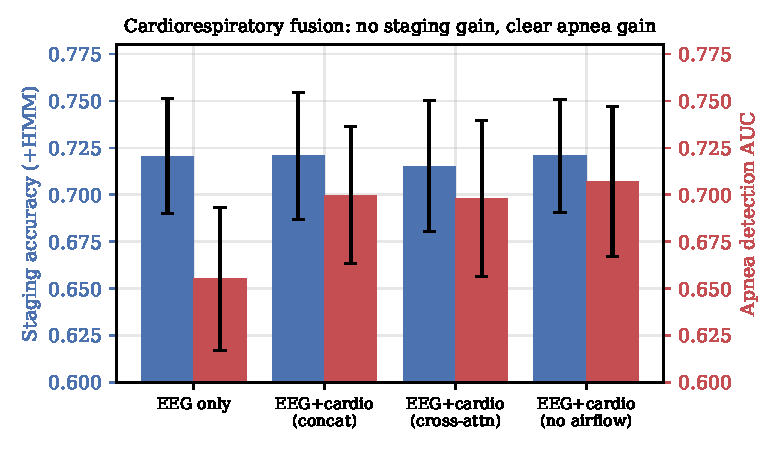
\includegraphics[width=0.94\columnwidth]{figures/fig_mm_ablation.pdf}
\caption{Effect of the cardiorespiratory stream. Staging accuracy (blue) stays at its full
level while respiratory-event AUC (red) rises sharply once the cardiorespiratory channels are
read. Error bars are fold standard deviations.}
\label{fig:ablationfig}
\end{figure}

\begin{table*}[t]
\caption{The proposed multimodal multi-task model in full, ten-fold patient-independent, and
the effect of the cardiorespiratory stream. Staging is at the hidden-Markov operating point;
per-class values are F1. The respiratory task is scored by AUC and average precision (AP).
Fold standard deviations in parentheses for the headline metrics.}
\label{tab:ablate}
\centering
\setlength{\tabcolsep}{5pt}
\begin{tabular}{lccc ccccc cc}
\toprule
 & \multicolumn{3}{c}{Staging} & \multicolumn{5}{c}{Per-class F1\,$\uparrow$} & \multicolumn{2}{c}{Respiratory}\\
\cmidrule(lr){2-4}\cmidrule(lr){5-9}\cmidrule(lr){10-11}
Variant & Acc\,$\uparrow$ & mF1\,$\uparrow$ & $\kappa$\,$\uparrow$ & W & N1 & N2 & N3 & R & AUC\,$\uparrow$ & AP\,$\uparrow$ \\
\midrule
Neural only              & 0.721\,(.031) & 0.635 & 0.603 & 0.77 & 0.24 & 0.78 & 0.68 & 0.70 & 0.655\,(.038) & 0.243 \\
Neural + cardio (concat) & 0.721\,(.034) & 0.645 & 0.606 & 0.77 & 0.27 & 0.78 & 0.68 & 0.72 & \textbf{0.700}\,(.037) & \textbf{0.333} \\
Neural + cardio (attention) & 0.715\,(.035) & 0.636 & 0.600 & 0.76 & 0.25 & 0.78 & 0.66 & 0.72 & 0.698\,(.042) & 0.324 \\
$\;$ airflow removed     & 0.721\,(.030) & 0.649 & 0.609 & 0.77 & 0.29 & 0.78 & 0.67 & 0.74 & 0.707\,(.040) & 0.328 \\
\bottomrule
\end{tabular}
\end{table*}

\subsection{Physiological Validity of the Respiratory Read-out}
\label{sec:noflow}
Because the events were scored from airflow, a model that keyed on the airflow channel would
be right for a trivial reason. We remove the two airflow features and test again. Detection is
not merely preserved, it is marginally higher, at $\noflowAuc$ AUC (Table~\ref{tab:ablate},
last row). The model therefore does not lean on the labeling signal. It reads the fall in
blood oxygen, the straining of the chest and abdomen, the beat-to-beat change in the heart, and
the cortical arousal that ends the event. This is the useful regime, because it detects the
bodily consequences of disordered breathing rather than repeating a measurement a technician
has already made.

\subsection{Model Complexity and Capability}
\begin{figure}[t]
\centering
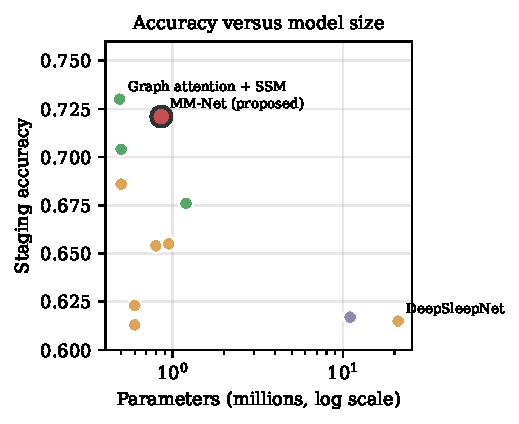
\includegraphics[width=0.92\columnwidth]{figures/fig_efficiency.pdf}
\caption{Staging accuracy against model size. The proposed model reaches top-band accuracy
with under a million parameters, an order of magnitude smaller than the raw-signal networks,
and is the only point that also detects respiratory events.}
\label{fig:efficiency}
\end{figure}
Table~\ref{tab:cost} sets the proposed model beside representative alternatives on size and
capability. A single compact network, under a million parameters and an order of magnitude
smaller than the raw-signal transformers, delivers both a competitive stage and a respiratory
read-out from one pass over the recording. None of the staging-only models, at any size, can
supply the second output.

\begin{table}[t]
\caption{Model size and clinical capability. The proposed model is compact and is the only one
that produces both a stage and a respiratory-event label.}
\label{tab:cost}
\centering
\setlength{\tabcolsep}{4pt}
\begin{tabular}{lccc}
\toprule
Model & Input & Params\,$\downarrow$ & Outputs \\
\midrule
CNN-ResNet18~\cite{maiti2026isleeps}      & 1\,EEG      & $\sim$11\,M & stage \\
DeepSleepNet~\cite{supratak2017deepsleepnet} & 1\,EEG   & $\sim$21\,M & stage \\
Feature-sequence BiLSTM                   & 7\,ch feat  & 1.2\,M      & stage \\
Graph attention + SSM                     & 7\,ch feat  & 0.49\,M     & stage \\
Raw multimodal CNN                        & 14\,ch      & 0.95\,M     & stage + apnea \\
\textbf{MM-Net (proposed)}                & 14\,ch feat & \textbf{0.86\,M} & \textbf{stage + apnea} \\
\bottomrule
\end{tabular}
\end{table}

%=====================================================================
\section{Discussion}
The result is a single model that reads the whole sleeping body and speaks to two clinical
questions at once, in the population where both matter. Across fifteen architectures, staging
accuracy on this cohort saturates near $0.72$ to $0.75$, and the proposed model sits inside
that top band while adding a respiratory capability the staging models lack. The respiratory
read-out is not a by-product of the label. It survives deletion of the airflow channel and
rests on oxygen desaturation, effort, and arousal, the same signs a physician reads at the
bedside.

The study also draws a clean physiological line. The cortical channels carry sleep staging, and
the cardiorespiratory channels carry breathing, and the model places each where it belongs
rather than blurring them. That the neural and multimodal variants stage alike is not a
shortfall; it is the correct outcome, and it tells us the second modality is adding a genuinely
new capability rather than reshuffling the first. We view this separation as a strength for
clinical use, because a reader can trust that the respiratory output reflects breathing and the
staging output reflects the brain.

Two directions follow naturally. Event-level metrics, such as sensitivity per event and false
alarms per hour, would sit beside the epoch-level AUC and speak more directly to a sleep
technician, and finer modeling of the breathing waveforms is likely to raise the respiratory
number further. Linking the multimodal representation to stroke severity and recovery is the
larger opportunity, and one the cardiorespiratory signal is well placed to serve.

%=====================================================================
\section{Conclusion}
We built a model that reads the full polysomnogram of stroke patients and, from one pass,
stages their sleep and detects their respiratory events. Against a benchmark of fifteen
architectures under patient-independent evaluation, it reaches $\mmAcc$ staging accuracy, in
the top band, and $\mmAuc$ respiratory-event AUC, and the respiratory read-out holds when the
airflow channel is removed, which shows it reads physiology rather than the label. Reading the
whole recording, not the brain alone, gives the model a second clinical voice in the population
that needs it most. Code and features are released.

%=====================================================================
\section*{Acknowledgment}
The authors thank the iSLEEPS investigators for releasing the corpus.

\bibliographystyle{IEEEtran}
\bibliography{references}

\end{document}
